\documentclass{article}

\usepackage{tikz}
\usetikzlibrary{matrix}

\begin{document}

\begin{figure}

\centering

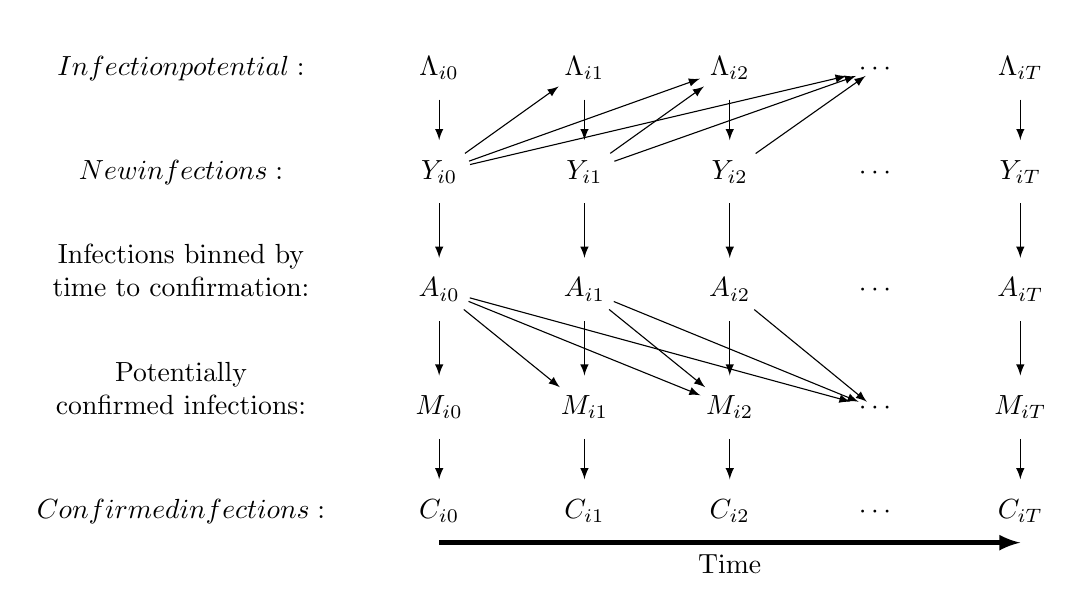
\begin{tikzpicture}

\matrix[
	matrix of math nodes,column sep=3em,
	row sep=1.5em,
	cells={nodes={circle,draw=none,minimum width=2.25em,inner sep=0pt}},
	column 1/.style={nodes={rectangle,draw=none}},
	column 5/.style={nodes={rectangle,draw=none}}
] (m) {
	\text{Infection potential}: &
	 \Lambda_{i0} & \Lambda_{i1} & \Lambda_{i2} & \cdots & \Lambda_{iT}\\
	\text{New infections}: & 
	  Y_{i0} & Y_{i1} & Y_{i2} & \cdots & Y_{iT} \\
	\node[align=center]{Infections binned by\\ time to confirmation:}; & 
	  \bm{A}_{i0} & \bm{A}_{i1} & \bm{A}_{i2} & \cdots & \bm{A}_{iT} \\
	\node[align=center]{Potentially \\ confirmed infections:}; & 
	  M_{i0} & M_{i1} & M_{i2}  & \cdots & M_{iT}\\
	\text{Confirmed infections}: & 
	  C_{i0} & C_{i1} & C_{i2} & \cdots & C_{iT} \\
};

\draw[-latex,ultra thick] (m-5-2.south) -- (m-5-6.south) node[midway,below]{Time};

\foreach \i in {2,3,4,6}
{
	\draw[-latex] (m-1-\i) -- (m-2-\i) node[pos=0.6,left]{};
	\draw[-latex] (m-2-\i) -- (m-3-\i) node[pos=0.6,left]{};
	\draw[-latex] (m-3-\i) -- (m-4-\i) node[pos=0.6,left]{};
	\draw[-latex] (m-4-\i) -- (m-5-\i) node[pos=0.6,left]{};
	
	\foreach \j in {2,3,4,5,6}
	{
		\pgfmathparse{int(\i + 4)}
		\ifnum\j>\i
			\ifnum\j<6
				\draw[-latex] (m-2-\i) -- (m-1-\j) node[pos=0.6,left]{};
				\draw[-latex] (m-3-\i) -- (m-4-\j) node[pos=0.6,left]{};
			\fi
		\fi
	}
}

\end{tikzpicture}

\caption{Simplified representation of the MERMAID framework. The number of infections $Y_{it}$ in region $i$ on day $t= 0, 1, ..., T$ depends on the current infection potential $\Lambda_{it}$, which is determined by the numbers of infections of previous days.  In practice, we assume that individuals are infectious for at most $m_{\Lambda}$ days, so that $\Lambda_{it}$ depends on $Y_{it'}$ only for $t-t' \leq m_{\Lambda}$ (not shown). New infections $Y_{it}$ that arose on day $t$ are binned by day that they are potentially confirmed; these binned infection counts are denoted by $\bm{A}_{it}$. The total number of individuals potentially confirmed on day $t$ is denoted by $M_{it}$, and of these only a subset of $C_{it}$ individuals are confirmed, and the remaining $M_{it}-C_{it}$ individuals are labeled as unascertained.  In practice, we assume that new infections are potentially confirmed at most $m_{A}$ days after infection, so that $M_{it}$ depends on $Y_{it'}$ only for $t-t' \leq m_{A}$ (not shown). For simplicity, serological survey outcomes and acquired immunity are not shown.}

\end{figure}

\end{document}
